\documentclass[10pt,a4paper,oneside,onecolumn]{article}
% PACKAGES
\usepackage[utf8]{inputenc}
\usepackage[english]{babel}
\usepackage[T1]{fontenc}
\usepackage{graphicx}
\usepackage{tikz}
\usepackage{pgf, booktabs, array}
% SETTINGS
\author{Ludovic.Charleux@univ-usmb.fr}
\title{Scientific plotter benchmark}
\date{2015}


\begin{document}
\maketitle
\tableofcontents
\newpage

\section{Simple Plot}

The goal is to plot data.csv in a 90 mm x 65 mm plot as follows.

\subsection{Matplotlib + PDF backend}
\begin{center}
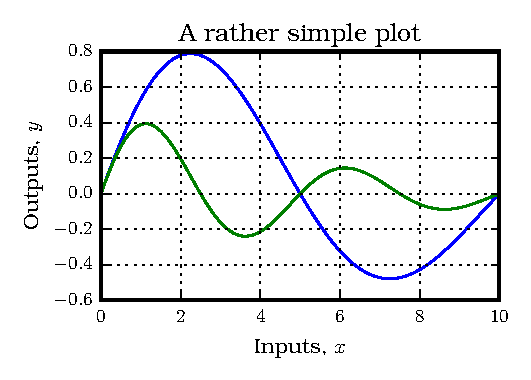
\includegraphics{simple_plot/mpl.pdf}
\end{center}

\subsection{Matplotlib + PGF backend}
\begin{center}
%% Creator: Matplotlib, PGF backend
%%
%% To include the figure in your LaTeX document, write
%%   \input{<filename>.pgf}
%%
%% Make sure the required packages are loaded in your preamble
%%   \usepackage{pgf}
%%
%% Figures using additional raster images can only be included by \input if
%% they are in the same directory as the main LaTeX file. For loading figures
%% from other directories you can use the `import` package
%%   \usepackage{import}
%% and then include the figures with
%%   \import{<path to file>}{<filename>.pgf}
%%
%% Matplotlib used the following preamble
%%   \usepackage{fontspec}
%%   \setmonofont{Courier}
%%
\begingroup%
\makeatletter%
\begin{pgfpicture}%
\pgfpathrectangle{\pgfpointorigin}{\pgfqpoint{3.543309in}{2.530935in}}%
\pgfusepath{use as bounding box, clip}%
\begin{pgfscope}%
\pgfsetbuttcap%
\pgfsetmiterjoin%
\definecolor{currentfill}{rgb}{1.000000,1.000000,1.000000}%
\pgfsetfillcolor{currentfill}%
\pgfsetlinewidth{0.000000pt}%
\definecolor{currentstroke}{rgb}{1.000000,1.000000,1.000000}%
\pgfsetstrokecolor{currentstroke}%
\pgfsetdash{}{0pt}%
\pgfpathmoveto{\pgfqpoint{0.000000in}{0.000000in}}%
\pgfpathlineto{\pgfqpoint{3.543309in}{0.000000in}}%
\pgfpathlineto{\pgfqpoint{3.543309in}{2.530935in}}%
\pgfpathlineto{\pgfqpoint{0.000000in}{2.530935in}}%
\pgfpathclose%
\pgfusepath{fill}%
\end{pgfscope}%
\begin{pgfscope}%
\pgfsetbuttcap%
\pgfsetmiterjoin%
\definecolor{currentfill}{rgb}{1.000000,1.000000,1.000000}%
\pgfsetfillcolor{currentfill}%
\pgfsetlinewidth{0.000000pt}%
\definecolor{currentstroke}{rgb}{0.000000,0.000000,0.000000}%
\pgfsetstrokecolor{currentstroke}%
\pgfsetstrokeopacity{0.000000}%
\pgfsetdash{}{0pt}%
\pgfpathmoveto{\pgfqpoint{0.672725in}{0.530800in}}%
\pgfpathlineto{\pgfqpoint{3.329313in}{0.530800in}}%
\pgfpathlineto{\pgfqpoint{3.329313in}{2.189698in}}%
\pgfpathlineto{\pgfqpoint{0.672725in}{2.189698in}}%
\pgfpathclose%
\pgfusepath{fill}%
\end{pgfscope}%
\begin{pgfscope}%
\pgfpathrectangle{\pgfqpoint{0.672725in}{0.530800in}}{\pgfqpoint{2.656588in}{1.658898in}} %
\pgfusepath{clip}%
\pgfsetrectcap%
\pgfsetroundjoin%
\pgfsetlinewidth{1.003750pt}%
\definecolor{currentstroke}{rgb}{0.000000,0.000000,1.000000}%
\pgfsetstrokecolor{currentstroke}%
\pgfsetdash{}{0pt}%
\pgfpathmoveto{\pgfqpoint{0.672725in}{1.241756in}}%
\pgfpathlineto{\pgfqpoint{0.699559in}{1.316154in}}%
\pgfpathlineto{\pgfqpoint{0.726394in}{1.388759in}}%
\pgfpathlineto{\pgfqpoint{0.753228in}{1.459312in}}%
\pgfpathlineto{\pgfqpoint{0.780062in}{1.527564in}}%
\pgfpathlineto{\pgfqpoint{0.806896in}{1.593283in}}%
\pgfpathlineto{\pgfqpoint{0.833730in}{1.656252in}}%
\pgfpathlineto{\pgfqpoint{0.860565in}{1.716266in}}%
\pgfpathlineto{\pgfqpoint{0.887399in}{1.773141in}}%
\pgfpathlineto{\pgfqpoint{0.914233in}{1.826707in}}%
\pgfpathlineto{\pgfqpoint{0.941067in}{1.876811in}}%
\pgfpathlineto{\pgfqpoint{0.967902in}{1.923317in}}%
\pgfpathlineto{\pgfqpoint{0.994736in}{1.966107in}}%
\pgfpathlineto{\pgfqpoint{1.021570in}{2.005081in}}%
\pgfpathlineto{\pgfqpoint{1.048404in}{2.040155in}}%
\pgfpathlineto{\pgfqpoint{1.075238in}{2.071265in}}%
\pgfpathlineto{\pgfqpoint{1.102073in}{2.098363in}}%
\pgfpathlineto{\pgfqpoint{1.128907in}{2.121417in}}%
\pgfpathlineto{\pgfqpoint{1.155741in}{2.140415in}}%
\pgfpathlineto{\pgfqpoint{1.182575in}{2.155360in}}%
\pgfpathlineto{\pgfqpoint{1.209410in}{2.166272in}}%
\pgfpathlineto{\pgfqpoint{1.236244in}{2.173187in}}%
\pgfpathlineto{\pgfqpoint{1.263078in}{2.176157in}}%
\pgfpathlineto{\pgfqpoint{1.289912in}{2.175249in}}%
\pgfpathlineto{\pgfqpoint{1.316746in}{2.170543in}}%
\pgfpathlineto{\pgfqpoint{1.343581in}{2.162135in}}%
\pgfpathlineto{\pgfqpoint{1.370415in}{2.150134in}}%
\pgfpathlineto{\pgfqpoint{1.397249in}{2.134660in}}%
\pgfpathlineto{\pgfqpoint{1.424083in}{2.115846in}}%
\pgfpathlineto{\pgfqpoint{1.450918in}{2.093836in}}%
\pgfpathlineto{\pgfqpoint{1.477752in}{2.068783in}}%
\pgfpathlineto{\pgfqpoint{1.504586in}{2.040851in}}%
\pgfpathlineto{\pgfqpoint{1.531420in}{2.010212in}}%
\pgfpathlineto{\pgfqpoint{1.558254in}{1.977044in}}%
\pgfpathlineto{\pgfqpoint{1.585089in}{1.941535in}}%
\pgfpathlineto{\pgfqpoint{1.611923in}{1.903876in}}%
\pgfpathlineto{\pgfqpoint{1.638757in}{1.864263in}}%
\pgfpathlineto{\pgfqpoint{1.665591in}{1.822899in}}%
\pgfpathlineto{\pgfqpoint{1.692426in}{1.779987in}}%
\pgfpathlineto{\pgfqpoint{1.719260in}{1.735733in}}%
\pgfpathlineto{\pgfqpoint{1.746094in}{1.690345in}}%
\pgfpathlineto{\pgfqpoint{1.772928in}{1.644031in}}%
\pgfpathlineto{\pgfqpoint{1.799763in}{1.597000in}}%
\pgfpathlineto{\pgfqpoint{1.826597in}{1.549457in}}%
\pgfpathlineto{\pgfqpoint{1.853431in}{1.501607in}}%
\pgfpathlineto{\pgfqpoint{1.880265in}{1.453652in}}%
\pgfpathlineto{\pgfqpoint{1.907099in}{1.405790in}}%
\pgfpathlineto{\pgfqpoint{1.933934in}{1.358215in}}%
\pgfpathlineto{\pgfqpoint{1.960768in}{1.311116in}}%
\pgfpathlineto{\pgfqpoint{1.987602in}{1.264675in}}%
\pgfpathlineto{\pgfqpoint{2.014436in}{1.219069in}}%
\pgfpathlineto{\pgfqpoint{2.041271in}{1.174467in}}%
\pgfpathlineto{\pgfqpoint{2.068105in}{1.131033in}}%
\pgfpathlineto{\pgfqpoint{2.094939in}{1.088920in}}%
\pgfpathlineto{\pgfqpoint{2.121773in}{1.048274in}}%
\pgfpathlineto{\pgfqpoint{2.148607in}{1.009232in}}%
\pgfpathlineto{\pgfqpoint{2.175442in}{0.971921in}}%
\pgfpathlineto{\pgfqpoint{2.202276in}{0.936459in}}%
\pgfpathlineto{\pgfqpoint{2.229110in}{0.902954in}}%
\pgfpathlineto{\pgfqpoint{2.255944in}{0.871503in}}%
\pgfpathlineto{\pgfqpoint{2.282779in}{0.842195in}}%
\pgfpathlineto{\pgfqpoint{2.309613in}{0.815107in}}%
\pgfpathlineto{\pgfqpoint{2.336447in}{0.790304in}}%
\pgfpathlineto{\pgfqpoint{2.363281in}{0.767842in}}%
\pgfpathlineto{\pgfqpoint{2.390115in}{0.747766in}}%
\pgfpathlineto{\pgfqpoint{2.416950in}{0.730111in}}%
\pgfpathlineto{\pgfqpoint{2.443784in}{0.714900in}}%
\pgfpathlineto{\pgfqpoint{2.470618in}{0.702146in}}%
\pgfpathlineto{\pgfqpoint{2.497452in}{0.691853in}}%
\pgfpathlineto{\pgfqpoint{2.524287in}{0.684014in}}%
\pgfpathlineto{\pgfqpoint{2.551121in}{0.678611in}}%
\pgfpathlineto{\pgfqpoint{2.577955in}{0.675618in}}%
\pgfpathlineto{\pgfqpoint{2.604789in}{0.674998in}}%
\pgfpathlineto{\pgfqpoint{2.631623in}{0.676707in}}%
\pgfpathlineto{\pgfqpoint{2.658458in}{0.680692in}}%
\pgfpathlineto{\pgfqpoint{2.685292in}{0.686890in}}%
\pgfpathlineto{\pgfqpoint{2.712126in}{0.695232in}}%
\pgfpathlineto{\pgfqpoint{2.738960in}{0.705641in}}%
\pgfpathlineto{\pgfqpoint{2.765795in}{0.718033in}}%
\pgfpathlineto{\pgfqpoint{2.792629in}{0.732317in}}%
\pgfpathlineto{\pgfqpoint{2.819463in}{0.748398in}}%
\pgfpathlineto{\pgfqpoint{2.846297in}{0.766174in}}%
\pgfpathlineto{\pgfqpoint{2.873131in}{0.785539in}}%
\pgfpathlineto{\pgfqpoint{2.899966in}{0.806380in}}%
\pgfpathlineto{\pgfqpoint{2.926800in}{0.828584in}}%
\pgfpathlineto{\pgfqpoint{2.953634in}{0.852033in}}%
\pgfpathlineto{\pgfqpoint{2.980468in}{0.876606in}}%
\pgfpathlineto{\pgfqpoint{3.007303in}{0.902180in}}%
\pgfpathlineto{\pgfqpoint{3.034137in}{0.928630in}}%
\pgfpathlineto{\pgfqpoint{3.060971in}{0.955831in}}%
\pgfpathlineto{\pgfqpoint{3.087805in}{0.983657in}}%
\pgfpathlineto{\pgfqpoint{3.114640in}{1.011981in}}%
\pgfpathlineto{\pgfqpoint{3.141474in}{1.040678in}}%
\pgfpathlineto{\pgfqpoint{3.168308in}{1.069622in}}%
\pgfpathlineto{\pgfqpoint{3.195142in}{1.098692in}}%
\pgfpathlineto{\pgfqpoint{3.221976in}{1.127765in}}%
\pgfpathlineto{\pgfqpoint{3.248811in}{1.156722in}}%
\pgfpathlineto{\pgfqpoint{3.275645in}{1.185447in}}%
\pgfpathlineto{\pgfqpoint{3.302479in}{1.213829in}}%
\pgfpathlineto{\pgfqpoint{3.329313in}{1.241756in}}%
\pgfusepath{stroke}%
\end{pgfscope}%
\begin{pgfscope}%
\pgfpathrectangle{\pgfqpoint{0.672725in}{0.530800in}}{\pgfqpoint{2.656588in}{1.658898in}} %
\pgfusepath{clip}%
\pgfsetrectcap%
\pgfsetroundjoin%
\pgfsetlinewidth{1.003750pt}%
\definecolor{currentstroke}{rgb}{0.000000,0.500000,0.000000}%
\pgfsetstrokecolor{currentstroke}%
\pgfsetdash{}{0pt}%
\pgfpathmoveto{\pgfqpoint{0.672725in}{1.241756in}}%
\pgfpathlineto{\pgfqpoint{0.699559in}{1.315258in}}%
\pgfpathlineto{\pgfqpoint{0.726394in}{1.384660in}}%
\pgfpathlineto{\pgfqpoint{0.753228in}{1.449004in}}%
\pgfpathlineto{\pgfqpoint{0.780062in}{1.507449in}}%
\pgfpathlineto{\pgfqpoint{0.806896in}{1.559284in}}%
\pgfpathlineto{\pgfqpoint{0.833730in}{1.603932in}}%
\pgfpathlineto{\pgfqpoint{0.860565in}{1.640956in}}%
\pgfpathlineto{\pgfqpoint{0.887399in}{1.670060in}}%
\pgfpathlineto{\pgfqpoint{0.914233in}{1.691086in}}%
\pgfpathlineto{\pgfqpoint{0.941067in}{1.704014in}}%
\pgfpathlineto{\pgfqpoint{0.967902in}{1.708957in}}%
\pgfpathlineto{\pgfqpoint{0.994736in}{1.706150in}}%
\pgfpathlineto{\pgfqpoint{1.021570in}{1.695945in}}%
\pgfpathlineto{\pgfqpoint{1.048404in}{1.678801in}}%
\pgfpathlineto{\pgfqpoint{1.075238in}{1.655270in}}%
\pgfpathlineto{\pgfqpoint{1.102073in}{1.625984in}}%
\pgfpathlineto{\pgfqpoint{1.128907in}{1.591646in}}%
\pgfpathlineto{\pgfqpoint{1.155741in}{1.553010in}}%
\pgfpathlineto{\pgfqpoint{1.182575in}{1.510872in}}%
\pgfpathlineto{\pgfqpoint{1.209410in}{1.466051in}}%
\pgfpathlineto{\pgfqpoint{1.236244in}{1.419378in}}%
\pgfpathlineto{\pgfqpoint{1.263078in}{1.371682in}}%
\pgfpathlineto{\pgfqpoint{1.289912in}{1.323773in}}%
\pgfpathlineto{\pgfqpoint{1.316746in}{1.276436in}}%
\pgfpathlineto{\pgfqpoint{1.343581in}{1.230413in}}%
\pgfpathlineto{\pgfqpoint{1.370415in}{1.186395in}}%
\pgfpathlineto{\pgfqpoint{1.397249in}{1.145015in}}%
\pgfpathlineto{\pgfqpoint{1.424083in}{1.106839in}}%
\pgfpathlineto{\pgfqpoint{1.450918in}{1.072355in}}%
\pgfpathlineto{\pgfqpoint{1.477752in}{1.041976in}}%
\pgfpathlineto{\pgfqpoint{1.504586in}{1.016030in}}%
\pgfpathlineto{\pgfqpoint{1.531420in}{0.994761in}}%
\pgfpathlineto{\pgfqpoint{1.558254in}{0.978328in}}%
\pgfpathlineto{\pgfqpoint{1.585089in}{0.966805in}}%
\pgfpathlineto{\pgfqpoint{1.611923in}{0.960184in}}%
\pgfpathlineto{\pgfqpoint{1.638757in}{0.958377in}}%
\pgfpathlineto{\pgfqpoint{1.665591in}{0.961224in}}%
\pgfpathlineto{\pgfqpoint{1.692426in}{0.968494in}}%
\pgfpathlineto{\pgfqpoint{1.719260in}{0.979895in}}%
\pgfpathlineto{\pgfqpoint{1.746094in}{0.995077in}}%
\pgfpathlineto{\pgfqpoint{1.772928in}{1.013647in}}%
\pgfpathlineto{\pgfqpoint{1.799763in}{1.035170in}}%
\pgfpathlineto{\pgfqpoint{1.826597in}{1.059181in}}%
\pgfpathlineto{\pgfqpoint{1.853431in}{1.085193in}}%
\pgfpathlineto{\pgfqpoint{1.880265in}{1.112707in}}%
\pgfpathlineto{\pgfqpoint{1.907099in}{1.141217in}}%
\pgfpathlineto{\pgfqpoint{1.933934in}{1.170224in}}%
\pgfpathlineto{\pgfqpoint{1.960768in}{1.199239in}}%
\pgfpathlineto{\pgfqpoint{1.987602in}{1.227793in}}%
\pgfpathlineto{\pgfqpoint{2.014436in}{1.255441in}}%
\pgfpathlineto{\pgfqpoint{2.041271in}{1.281774in}}%
\pgfpathlineto{\pgfqpoint{2.068105in}{1.306416in}}%
\pgfpathlineto{\pgfqpoint{2.094939in}{1.329038in}}%
\pgfpathlineto{\pgfqpoint{2.121773in}{1.349352in}}%
\pgfpathlineto{\pgfqpoint{2.148607in}{1.367122in}}%
\pgfpathlineto{\pgfqpoint{2.175442in}{1.382162in}}%
\pgfpathlineto{\pgfqpoint{2.202276in}{1.394336in}}%
\pgfpathlineto{\pgfqpoint{2.229110in}{1.403561in}}%
\pgfpathlineto{\pgfqpoint{2.255944in}{1.409804in}}%
\pgfpathlineto{\pgfqpoint{2.282779in}{1.413084in}}%
\pgfpathlineto{\pgfqpoint{2.309613in}{1.413463in}}%
\pgfpathlineto{\pgfqpoint{2.336447in}{1.411051in}}%
\pgfpathlineto{\pgfqpoint{2.363281in}{1.405997in}}%
\pgfpathlineto{\pgfqpoint{2.390115in}{1.398488in}}%
\pgfpathlineto{\pgfqpoint{2.416950in}{1.388742in}}%
\pgfpathlineto{\pgfqpoint{2.443784in}{1.377005in}}%
\pgfpathlineto{\pgfqpoint{2.470618in}{1.363546in}}%
\pgfpathlineto{\pgfqpoint{2.497452in}{1.348652in}}%
\pgfpathlineto{\pgfqpoint{2.524287in}{1.332618in}}%
\pgfpathlineto{\pgfqpoint{2.551121in}{1.315751in}}%
\pgfpathlineto{\pgfqpoint{2.577955in}{1.298355in}}%
\pgfpathlineto{\pgfqpoint{2.604789in}{1.280732in}}%
\pgfpathlineto{\pgfqpoint{2.631623in}{1.263178in}}%
\pgfpathlineto{\pgfqpoint{2.658458in}{1.245972in}}%
\pgfpathlineto{\pgfqpoint{2.685292in}{1.229379in}}%
\pgfpathlineto{\pgfqpoint{2.712126in}{1.213644in}}%
\pgfpathlineto{\pgfqpoint{2.738960in}{1.198986in}}%
\pgfpathlineto{\pgfqpoint{2.765795in}{1.185600in}}%
\pgfpathlineto{\pgfqpoint{2.792629in}{1.173652in}}%
\pgfpathlineto{\pgfqpoint{2.819463in}{1.163279in}}%
\pgfpathlineto{\pgfqpoint{2.846297in}{1.154585in}}%
\pgfpathlineto{\pgfqpoint{2.873131in}{1.147644in}}%
\pgfpathlineto{\pgfqpoint{2.899966in}{1.142501in}}%
\pgfpathlineto{\pgfqpoint{2.926800in}{1.139165in}}%
\pgfpathlineto{\pgfqpoint{2.953634in}{1.137621in}}%
\pgfpathlineto{\pgfqpoint{2.980468in}{1.137821in}}%
\pgfpathlineto{\pgfqpoint{3.007303in}{1.139694in}}%
\pgfpathlineto{\pgfqpoint{3.034137in}{1.143143in}}%
\pgfpathlineto{\pgfqpoint{3.060971in}{1.148050in}}%
\pgfpathlineto{\pgfqpoint{3.087805in}{1.154278in}}%
\pgfpathlineto{\pgfqpoint{3.114640in}{1.161673in}}%
\pgfpathlineto{\pgfqpoint{3.141474in}{1.170071in}}%
\pgfpathlineto{\pgfqpoint{3.168308in}{1.179295in}}%
\pgfpathlineto{\pgfqpoint{3.195142in}{1.189163in}}%
\pgfpathlineto{\pgfqpoint{3.221976in}{1.199492in}}%
\pgfpathlineto{\pgfqpoint{3.248811in}{1.210094in}}%
\pgfpathlineto{\pgfqpoint{3.275645in}{1.220789in}}%
\pgfpathlineto{\pgfqpoint{3.302479in}{1.231399in}}%
\pgfpathlineto{\pgfqpoint{3.329313in}{1.241756in}}%
\pgfusepath{stroke}%
\end{pgfscope}%
\begin{pgfscope}%
\pgfsetrectcap%
\pgfsetmiterjoin%
\pgfsetlinewidth{1.505625pt}%
\definecolor{currentstroke}{rgb}{0.000000,0.000000,0.000000}%
\pgfsetstrokecolor{currentstroke}%
\pgfsetdash{}{0pt}%
\pgfpathmoveto{\pgfqpoint{0.672725in}{2.189698in}}%
\pgfpathlineto{\pgfqpoint{3.329313in}{2.189698in}}%
\pgfusepath{stroke}%
\end{pgfscope}%
\begin{pgfscope}%
\pgfsetrectcap%
\pgfsetmiterjoin%
\pgfsetlinewidth{1.505625pt}%
\definecolor{currentstroke}{rgb}{0.000000,0.000000,0.000000}%
\pgfsetstrokecolor{currentstroke}%
\pgfsetdash{}{0pt}%
\pgfpathmoveto{\pgfqpoint{3.329313in}{0.530800in}}%
\pgfpathlineto{\pgfqpoint{3.329313in}{2.189698in}}%
\pgfusepath{stroke}%
\end{pgfscope}%
\begin{pgfscope}%
\pgfsetrectcap%
\pgfsetmiterjoin%
\pgfsetlinewidth{1.505625pt}%
\definecolor{currentstroke}{rgb}{0.000000,0.000000,0.000000}%
\pgfsetstrokecolor{currentstroke}%
\pgfsetdash{}{0pt}%
\pgfpathmoveto{\pgfqpoint{0.672725in}{0.530800in}}%
\pgfpathlineto{\pgfqpoint{3.329313in}{0.530800in}}%
\pgfusepath{stroke}%
\end{pgfscope}%
\begin{pgfscope}%
\pgfsetrectcap%
\pgfsetmiterjoin%
\pgfsetlinewidth{1.505625pt}%
\definecolor{currentstroke}{rgb}{0.000000,0.000000,0.000000}%
\pgfsetstrokecolor{currentstroke}%
\pgfsetdash{}{0pt}%
\pgfpathmoveto{\pgfqpoint{0.672725in}{0.530800in}}%
\pgfpathlineto{\pgfqpoint{0.672725in}{2.189698in}}%
\pgfusepath{stroke}%
\end{pgfscope}%
\begin{pgfscope}%
\pgfpathrectangle{\pgfqpoint{0.672725in}{0.530800in}}{\pgfqpoint{2.656588in}{1.658898in}} %
\pgfusepath{clip}%
\pgfsetbuttcap%
\pgfsetroundjoin%
\pgfsetlinewidth{0.501875pt}%
\definecolor{currentstroke}{rgb}{0.000000,0.000000,0.000000}%
\pgfsetstrokecolor{currentstroke}%
\pgfsetdash{{1.000000pt}{3.000000pt}}{0.000000pt}%
\pgfpathmoveto{\pgfqpoint{0.672725in}{0.530800in}}%
\pgfpathlineto{\pgfqpoint{0.672725in}{2.189698in}}%
\pgfusepath{stroke}%
\end{pgfscope}%
\begin{pgfscope}%
\pgfsetbuttcap%
\pgfsetroundjoin%
\definecolor{currentfill}{rgb}{0.000000,0.000000,0.000000}%
\pgfsetfillcolor{currentfill}%
\pgfsetlinewidth{0.501875pt}%
\definecolor{currentstroke}{rgb}{0.000000,0.000000,0.000000}%
\pgfsetstrokecolor{currentstroke}%
\pgfsetdash{}{0pt}%
\pgfsys@defobject{currentmarker}{\pgfqpoint{0.000000in}{0.000000in}}{\pgfqpoint{0.000000in}{0.055556in}}{%
\pgfpathmoveto{\pgfqpoint{0.000000in}{0.000000in}}%
\pgfpathlineto{\pgfqpoint{0.000000in}{0.055556in}}%
\pgfusepath{stroke,fill}%
}%
\begin{pgfscope}%
\pgfsys@transformshift{0.672725in}{0.530800in}%
\pgfsys@useobject{currentmarker}{}%
\end{pgfscope}%
\end{pgfscope}%
\begin{pgfscope}%
\pgfsetbuttcap%
\pgfsetroundjoin%
\definecolor{currentfill}{rgb}{0.000000,0.000000,0.000000}%
\pgfsetfillcolor{currentfill}%
\pgfsetlinewidth{0.501875pt}%
\definecolor{currentstroke}{rgb}{0.000000,0.000000,0.000000}%
\pgfsetstrokecolor{currentstroke}%
\pgfsetdash{}{0pt}%
\pgfsys@defobject{currentmarker}{\pgfqpoint{0.000000in}{-0.055556in}}{\pgfqpoint{0.000000in}{0.000000in}}{%
\pgfpathmoveto{\pgfqpoint{0.000000in}{0.000000in}}%
\pgfpathlineto{\pgfqpoint{0.000000in}{-0.055556in}}%
\pgfusepath{stroke,fill}%
}%
\begin{pgfscope}%
\pgfsys@transformshift{0.672725in}{2.189698in}%
\pgfsys@useobject{currentmarker}{}%
\end{pgfscope}%
\end{pgfscope}%
\begin{pgfscope}%
\pgftext[x=0.672725in,y=0.475245in,,top]{\rmfamily\fontsize{9.000000}{10.800000}\selectfont \(\displaystyle 0\)}%
\end{pgfscope}%
\begin{pgfscope}%
\pgfpathrectangle{\pgfqpoint{0.672725in}{0.530800in}}{\pgfqpoint{2.656588in}{1.658898in}} %
\pgfusepath{clip}%
\pgfsetbuttcap%
\pgfsetroundjoin%
\pgfsetlinewidth{0.501875pt}%
\definecolor{currentstroke}{rgb}{0.000000,0.000000,0.000000}%
\pgfsetstrokecolor{currentstroke}%
\pgfsetdash{{1.000000pt}{3.000000pt}}{0.000000pt}%
\pgfpathmoveto{\pgfqpoint{1.204043in}{0.530800in}}%
\pgfpathlineto{\pgfqpoint{1.204043in}{2.189698in}}%
\pgfusepath{stroke}%
\end{pgfscope}%
\begin{pgfscope}%
\pgfsetbuttcap%
\pgfsetroundjoin%
\definecolor{currentfill}{rgb}{0.000000,0.000000,0.000000}%
\pgfsetfillcolor{currentfill}%
\pgfsetlinewidth{0.501875pt}%
\definecolor{currentstroke}{rgb}{0.000000,0.000000,0.000000}%
\pgfsetstrokecolor{currentstroke}%
\pgfsetdash{}{0pt}%
\pgfsys@defobject{currentmarker}{\pgfqpoint{0.000000in}{0.000000in}}{\pgfqpoint{0.000000in}{0.055556in}}{%
\pgfpathmoveto{\pgfqpoint{0.000000in}{0.000000in}}%
\pgfpathlineto{\pgfqpoint{0.000000in}{0.055556in}}%
\pgfusepath{stroke,fill}%
}%
\begin{pgfscope}%
\pgfsys@transformshift{1.204043in}{0.530800in}%
\pgfsys@useobject{currentmarker}{}%
\end{pgfscope}%
\end{pgfscope}%
\begin{pgfscope}%
\pgfsetbuttcap%
\pgfsetroundjoin%
\definecolor{currentfill}{rgb}{0.000000,0.000000,0.000000}%
\pgfsetfillcolor{currentfill}%
\pgfsetlinewidth{0.501875pt}%
\definecolor{currentstroke}{rgb}{0.000000,0.000000,0.000000}%
\pgfsetstrokecolor{currentstroke}%
\pgfsetdash{}{0pt}%
\pgfsys@defobject{currentmarker}{\pgfqpoint{0.000000in}{-0.055556in}}{\pgfqpoint{0.000000in}{0.000000in}}{%
\pgfpathmoveto{\pgfqpoint{0.000000in}{0.000000in}}%
\pgfpathlineto{\pgfqpoint{0.000000in}{-0.055556in}}%
\pgfusepath{stroke,fill}%
}%
\begin{pgfscope}%
\pgfsys@transformshift{1.204043in}{2.189698in}%
\pgfsys@useobject{currentmarker}{}%
\end{pgfscope}%
\end{pgfscope}%
\begin{pgfscope}%
\pgftext[x=1.204043in,y=0.475245in,,top]{\rmfamily\fontsize{9.000000}{10.800000}\selectfont \(\displaystyle 2\)}%
\end{pgfscope}%
\begin{pgfscope}%
\pgfpathrectangle{\pgfqpoint{0.672725in}{0.530800in}}{\pgfqpoint{2.656588in}{1.658898in}} %
\pgfusepath{clip}%
\pgfsetbuttcap%
\pgfsetroundjoin%
\pgfsetlinewidth{0.501875pt}%
\definecolor{currentstroke}{rgb}{0.000000,0.000000,0.000000}%
\pgfsetstrokecolor{currentstroke}%
\pgfsetdash{{1.000000pt}{3.000000pt}}{0.000000pt}%
\pgfpathmoveto{\pgfqpoint{1.735360in}{0.530800in}}%
\pgfpathlineto{\pgfqpoint{1.735360in}{2.189698in}}%
\pgfusepath{stroke}%
\end{pgfscope}%
\begin{pgfscope}%
\pgfsetbuttcap%
\pgfsetroundjoin%
\definecolor{currentfill}{rgb}{0.000000,0.000000,0.000000}%
\pgfsetfillcolor{currentfill}%
\pgfsetlinewidth{0.501875pt}%
\definecolor{currentstroke}{rgb}{0.000000,0.000000,0.000000}%
\pgfsetstrokecolor{currentstroke}%
\pgfsetdash{}{0pt}%
\pgfsys@defobject{currentmarker}{\pgfqpoint{0.000000in}{0.000000in}}{\pgfqpoint{0.000000in}{0.055556in}}{%
\pgfpathmoveto{\pgfqpoint{0.000000in}{0.000000in}}%
\pgfpathlineto{\pgfqpoint{0.000000in}{0.055556in}}%
\pgfusepath{stroke,fill}%
}%
\begin{pgfscope}%
\pgfsys@transformshift{1.735360in}{0.530800in}%
\pgfsys@useobject{currentmarker}{}%
\end{pgfscope}%
\end{pgfscope}%
\begin{pgfscope}%
\pgfsetbuttcap%
\pgfsetroundjoin%
\definecolor{currentfill}{rgb}{0.000000,0.000000,0.000000}%
\pgfsetfillcolor{currentfill}%
\pgfsetlinewidth{0.501875pt}%
\definecolor{currentstroke}{rgb}{0.000000,0.000000,0.000000}%
\pgfsetstrokecolor{currentstroke}%
\pgfsetdash{}{0pt}%
\pgfsys@defobject{currentmarker}{\pgfqpoint{0.000000in}{-0.055556in}}{\pgfqpoint{0.000000in}{0.000000in}}{%
\pgfpathmoveto{\pgfqpoint{0.000000in}{0.000000in}}%
\pgfpathlineto{\pgfqpoint{0.000000in}{-0.055556in}}%
\pgfusepath{stroke,fill}%
}%
\begin{pgfscope}%
\pgfsys@transformshift{1.735360in}{2.189698in}%
\pgfsys@useobject{currentmarker}{}%
\end{pgfscope}%
\end{pgfscope}%
\begin{pgfscope}%
\pgftext[x=1.735360in,y=0.475245in,,top]{\rmfamily\fontsize{9.000000}{10.800000}\selectfont \(\displaystyle 4\)}%
\end{pgfscope}%
\begin{pgfscope}%
\pgfpathrectangle{\pgfqpoint{0.672725in}{0.530800in}}{\pgfqpoint{2.656588in}{1.658898in}} %
\pgfusepath{clip}%
\pgfsetbuttcap%
\pgfsetroundjoin%
\pgfsetlinewidth{0.501875pt}%
\definecolor{currentstroke}{rgb}{0.000000,0.000000,0.000000}%
\pgfsetstrokecolor{currentstroke}%
\pgfsetdash{{1.000000pt}{3.000000pt}}{0.000000pt}%
\pgfpathmoveto{\pgfqpoint{2.266678in}{0.530800in}}%
\pgfpathlineto{\pgfqpoint{2.266678in}{2.189698in}}%
\pgfusepath{stroke}%
\end{pgfscope}%
\begin{pgfscope}%
\pgfsetbuttcap%
\pgfsetroundjoin%
\definecolor{currentfill}{rgb}{0.000000,0.000000,0.000000}%
\pgfsetfillcolor{currentfill}%
\pgfsetlinewidth{0.501875pt}%
\definecolor{currentstroke}{rgb}{0.000000,0.000000,0.000000}%
\pgfsetstrokecolor{currentstroke}%
\pgfsetdash{}{0pt}%
\pgfsys@defobject{currentmarker}{\pgfqpoint{0.000000in}{0.000000in}}{\pgfqpoint{0.000000in}{0.055556in}}{%
\pgfpathmoveto{\pgfqpoint{0.000000in}{0.000000in}}%
\pgfpathlineto{\pgfqpoint{0.000000in}{0.055556in}}%
\pgfusepath{stroke,fill}%
}%
\begin{pgfscope}%
\pgfsys@transformshift{2.266678in}{0.530800in}%
\pgfsys@useobject{currentmarker}{}%
\end{pgfscope}%
\end{pgfscope}%
\begin{pgfscope}%
\pgfsetbuttcap%
\pgfsetroundjoin%
\definecolor{currentfill}{rgb}{0.000000,0.000000,0.000000}%
\pgfsetfillcolor{currentfill}%
\pgfsetlinewidth{0.501875pt}%
\definecolor{currentstroke}{rgb}{0.000000,0.000000,0.000000}%
\pgfsetstrokecolor{currentstroke}%
\pgfsetdash{}{0pt}%
\pgfsys@defobject{currentmarker}{\pgfqpoint{0.000000in}{-0.055556in}}{\pgfqpoint{0.000000in}{0.000000in}}{%
\pgfpathmoveto{\pgfqpoint{0.000000in}{0.000000in}}%
\pgfpathlineto{\pgfqpoint{0.000000in}{-0.055556in}}%
\pgfusepath{stroke,fill}%
}%
\begin{pgfscope}%
\pgfsys@transformshift{2.266678in}{2.189698in}%
\pgfsys@useobject{currentmarker}{}%
\end{pgfscope}%
\end{pgfscope}%
\begin{pgfscope}%
\pgftext[x=2.266678in,y=0.475245in,,top]{\rmfamily\fontsize{9.000000}{10.800000}\selectfont \(\displaystyle 6\)}%
\end{pgfscope}%
\begin{pgfscope}%
\pgfpathrectangle{\pgfqpoint{0.672725in}{0.530800in}}{\pgfqpoint{2.656588in}{1.658898in}} %
\pgfusepath{clip}%
\pgfsetbuttcap%
\pgfsetroundjoin%
\pgfsetlinewidth{0.501875pt}%
\definecolor{currentstroke}{rgb}{0.000000,0.000000,0.000000}%
\pgfsetstrokecolor{currentstroke}%
\pgfsetdash{{1.000000pt}{3.000000pt}}{0.000000pt}%
\pgfpathmoveto{\pgfqpoint{2.797996in}{0.530800in}}%
\pgfpathlineto{\pgfqpoint{2.797996in}{2.189698in}}%
\pgfusepath{stroke}%
\end{pgfscope}%
\begin{pgfscope}%
\pgfsetbuttcap%
\pgfsetroundjoin%
\definecolor{currentfill}{rgb}{0.000000,0.000000,0.000000}%
\pgfsetfillcolor{currentfill}%
\pgfsetlinewidth{0.501875pt}%
\definecolor{currentstroke}{rgb}{0.000000,0.000000,0.000000}%
\pgfsetstrokecolor{currentstroke}%
\pgfsetdash{}{0pt}%
\pgfsys@defobject{currentmarker}{\pgfqpoint{0.000000in}{0.000000in}}{\pgfqpoint{0.000000in}{0.055556in}}{%
\pgfpathmoveto{\pgfqpoint{0.000000in}{0.000000in}}%
\pgfpathlineto{\pgfqpoint{0.000000in}{0.055556in}}%
\pgfusepath{stroke,fill}%
}%
\begin{pgfscope}%
\pgfsys@transformshift{2.797996in}{0.530800in}%
\pgfsys@useobject{currentmarker}{}%
\end{pgfscope}%
\end{pgfscope}%
\begin{pgfscope}%
\pgfsetbuttcap%
\pgfsetroundjoin%
\definecolor{currentfill}{rgb}{0.000000,0.000000,0.000000}%
\pgfsetfillcolor{currentfill}%
\pgfsetlinewidth{0.501875pt}%
\definecolor{currentstroke}{rgb}{0.000000,0.000000,0.000000}%
\pgfsetstrokecolor{currentstroke}%
\pgfsetdash{}{0pt}%
\pgfsys@defobject{currentmarker}{\pgfqpoint{0.000000in}{-0.055556in}}{\pgfqpoint{0.000000in}{0.000000in}}{%
\pgfpathmoveto{\pgfqpoint{0.000000in}{0.000000in}}%
\pgfpathlineto{\pgfqpoint{0.000000in}{-0.055556in}}%
\pgfusepath{stroke,fill}%
}%
\begin{pgfscope}%
\pgfsys@transformshift{2.797996in}{2.189698in}%
\pgfsys@useobject{currentmarker}{}%
\end{pgfscope}%
\end{pgfscope}%
\begin{pgfscope}%
\pgftext[x=2.797996in,y=0.475245in,,top]{\rmfamily\fontsize{9.000000}{10.800000}\selectfont \(\displaystyle 8\)}%
\end{pgfscope}%
\begin{pgfscope}%
\pgfpathrectangle{\pgfqpoint{0.672725in}{0.530800in}}{\pgfqpoint{2.656588in}{1.658898in}} %
\pgfusepath{clip}%
\pgfsetbuttcap%
\pgfsetroundjoin%
\pgfsetlinewidth{0.501875pt}%
\definecolor{currentstroke}{rgb}{0.000000,0.000000,0.000000}%
\pgfsetstrokecolor{currentstroke}%
\pgfsetdash{{1.000000pt}{3.000000pt}}{0.000000pt}%
\pgfpathmoveto{\pgfqpoint{3.329313in}{0.530800in}}%
\pgfpathlineto{\pgfqpoint{3.329313in}{2.189698in}}%
\pgfusepath{stroke}%
\end{pgfscope}%
\begin{pgfscope}%
\pgfsetbuttcap%
\pgfsetroundjoin%
\definecolor{currentfill}{rgb}{0.000000,0.000000,0.000000}%
\pgfsetfillcolor{currentfill}%
\pgfsetlinewidth{0.501875pt}%
\definecolor{currentstroke}{rgb}{0.000000,0.000000,0.000000}%
\pgfsetstrokecolor{currentstroke}%
\pgfsetdash{}{0pt}%
\pgfsys@defobject{currentmarker}{\pgfqpoint{0.000000in}{0.000000in}}{\pgfqpoint{0.000000in}{0.055556in}}{%
\pgfpathmoveto{\pgfqpoint{0.000000in}{0.000000in}}%
\pgfpathlineto{\pgfqpoint{0.000000in}{0.055556in}}%
\pgfusepath{stroke,fill}%
}%
\begin{pgfscope}%
\pgfsys@transformshift{3.329313in}{0.530800in}%
\pgfsys@useobject{currentmarker}{}%
\end{pgfscope}%
\end{pgfscope}%
\begin{pgfscope}%
\pgfsetbuttcap%
\pgfsetroundjoin%
\definecolor{currentfill}{rgb}{0.000000,0.000000,0.000000}%
\pgfsetfillcolor{currentfill}%
\pgfsetlinewidth{0.501875pt}%
\definecolor{currentstroke}{rgb}{0.000000,0.000000,0.000000}%
\pgfsetstrokecolor{currentstroke}%
\pgfsetdash{}{0pt}%
\pgfsys@defobject{currentmarker}{\pgfqpoint{0.000000in}{-0.055556in}}{\pgfqpoint{0.000000in}{0.000000in}}{%
\pgfpathmoveto{\pgfqpoint{0.000000in}{0.000000in}}%
\pgfpathlineto{\pgfqpoint{0.000000in}{-0.055556in}}%
\pgfusepath{stroke,fill}%
}%
\begin{pgfscope}%
\pgfsys@transformshift{3.329313in}{2.189698in}%
\pgfsys@useobject{currentmarker}{}%
\end{pgfscope}%
\end{pgfscope}%
\begin{pgfscope}%
\pgftext[x=3.329313in,y=0.475245in,,top]{\rmfamily\fontsize{9.000000}{10.800000}\selectfont \(\displaystyle 10\)}%
\end{pgfscope}%
\begin{pgfscope}%
\pgftext[x=2.001019in,y=0.294800in,,top]{\rmfamily\fontsize{10.000000}{12.000000}\selectfont Inputs,  \(\displaystyle x\)}%
\end{pgfscope}%
\begin{pgfscope}%
\pgfpathrectangle{\pgfqpoint{0.672725in}{0.530800in}}{\pgfqpoint{2.656588in}{1.658898in}} %
\pgfusepath{clip}%
\pgfsetbuttcap%
\pgfsetroundjoin%
\pgfsetlinewidth{0.501875pt}%
\definecolor{currentstroke}{rgb}{0.000000,0.000000,0.000000}%
\pgfsetstrokecolor{currentstroke}%
\pgfsetdash{{1.000000pt}{3.000000pt}}{0.000000pt}%
\pgfpathmoveto{\pgfqpoint{0.672725in}{0.530800in}}%
\pgfpathlineto{\pgfqpoint{3.329313in}{0.530800in}}%
\pgfusepath{stroke}%
\end{pgfscope}%
\begin{pgfscope}%
\pgfsetbuttcap%
\pgfsetroundjoin%
\definecolor{currentfill}{rgb}{0.000000,0.000000,0.000000}%
\pgfsetfillcolor{currentfill}%
\pgfsetlinewidth{0.501875pt}%
\definecolor{currentstroke}{rgb}{0.000000,0.000000,0.000000}%
\pgfsetstrokecolor{currentstroke}%
\pgfsetdash{}{0pt}%
\pgfsys@defobject{currentmarker}{\pgfqpoint{0.000000in}{0.000000in}}{\pgfqpoint{0.055556in}{0.000000in}}{%
\pgfpathmoveto{\pgfqpoint{0.000000in}{0.000000in}}%
\pgfpathlineto{\pgfqpoint{0.055556in}{0.000000in}}%
\pgfusepath{stroke,fill}%
}%
\begin{pgfscope}%
\pgfsys@transformshift{0.672725in}{0.530800in}%
\pgfsys@useobject{currentmarker}{}%
\end{pgfscope}%
\end{pgfscope}%
\begin{pgfscope}%
\pgfsetbuttcap%
\pgfsetroundjoin%
\definecolor{currentfill}{rgb}{0.000000,0.000000,0.000000}%
\pgfsetfillcolor{currentfill}%
\pgfsetlinewidth{0.501875pt}%
\definecolor{currentstroke}{rgb}{0.000000,0.000000,0.000000}%
\pgfsetstrokecolor{currentstroke}%
\pgfsetdash{}{0pt}%
\pgfsys@defobject{currentmarker}{\pgfqpoint{-0.055556in}{0.000000in}}{\pgfqpoint{0.000000in}{0.000000in}}{%
\pgfpathmoveto{\pgfqpoint{0.000000in}{0.000000in}}%
\pgfpathlineto{\pgfqpoint{-0.055556in}{0.000000in}}%
\pgfusepath{stroke,fill}%
}%
\begin{pgfscope}%
\pgfsys@transformshift{3.329313in}{0.530800in}%
\pgfsys@useobject{currentmarker}{}%
\end{pgfscope}%
\end{pgfscope}%
\begin{pgfscope}%
\pgftext[x=0.617170in,y=0.530800in,right,]{\rmfamily\fontsize{9.000000}{10.800000}\selectfont \(\displaystyle -0.6\)}%
\end{pgfscope}%
\begin{pgfscope}%
\pgfpathrectangle{\pgfqpoint{0.672725in}{0.530800in}}{\pgfqpoint{2.656588in}{1.658898in}} %
\pgfusepath{clip}%
\pgfsetbuttcap%
\pgfsetroundjoin%
\pgfsetlinewidth{0.501875pt}%
\definecolor{currentstroke}{rgb}{0.000000,0.000000,0.000000}%
\pgfsetstrokecolor{currentstroke}%
\pgfsetdash{{1.000000pt}{3.000000pt}}{0.000000pt}%
\pgfpathmoveto{\pgfqpoint{0.672725in}{0.767786in}}%
\pgfpathlineto{\pgfqpoint{3.329313in}{0.767786in}}%
\pgfusepath{stroke}%
\end{pgfscope}%
\begin{pgfscope}%
\pgfsetbuttcap%
\pgfsetroundjoin%
\definecolor{currentfill}{rgb}{0.000000,0.000000,0.000000}%
\pgfsetfillcolor{currentfill}%
\pgfsetlinewidth{0.501875pt}%
\definecolor{currentstroke}{rgb}{0.000000,0.000000,0.000000}%
\pgfsetstrokecolor{currentstroke}%
\pgfsetdash{}{0pt}%
\pgfsys@defobject{currentmarker}{\pgfqpoint{0.000000in}{0.000000in}}{\pgfqpoint{0.055556in}{0.000000in}}{%
\pgfpathmoveto{\pgfqpoint{0.000000in}{0.000000in}}%
\pgfpathlineto{\pgfqpoint{0.055556in}{0.000000in}}%
\pgfusepath{stroke,fill}%
}%
\begin{pgfscope}%
\pgfsys@transformshift{0.672725in}{0.767786in}%
\pgfsys@useobject{currentmarker}{}%
\end{pgfscope}%
\end{pgfscope}%
\begin{pgfscope}%
\pgfsetbuttcap%
\pgfsetroundjoin%
\definecolor{currentfill}{rgb}{0.000000,0.000000,0.000000}%
\pgfsetfillcolor{currentfill}%
\pgfsetlinewidth{0.501875pt}%
\definecolor{currentstroke}{rgb}{0.000000,0.000000,0.000000}%
\pgfsetstrokecolor{currentstroke}%
\pgfsetdash{}{0pt}%
\pgfsys@defobject{currentmarker}{\pgfqpoint{-0.055556in}{0.000000in}}{\pgfqpoint{0.000000in}{0.000000in}}{%
\pgfpathmoveto{\pgfqpoint{0.000000in}{0.000000in}}%
\pgfpathlineto{\pgfqpoint{-0.055556in}{0.000000in}}%
\pgfusepath{stroke,fill}%
}%
\begin{pgfscope}%
\pgfsys@transformshift{3.329313in}{0.767786in}%
\pgfsys@useobject{currentmarker}{}%
\end{pgfscope}%
\end{pgfscope}%
\begin{pgfscope}%
\pgftext[x=0.617170in,y=0.767786in,right,]{\rmfamily\fontsize{9.000000}{10.800000}\selectfont \(\displaystyle -0.4\)}%
\end{pgfscope}%
\begin{pgfscope}%
\pgfpathrectangle{\pgfqpoint{0.672725in}{0.530800in}}{\pgfqpoint{2.656588in}{1.658898in}} %
\pgfusepath{clip}%
\pgfsetbuttcap%
\pgfsetroundjoin%
\pgfsetlinewidth{0.501875pt}%
\definecolor{currentstroke}{rgb}{0.000000,0.000000,0.000000}%
\pgfsetstrokecolor{currentstroke}%
\pgfsetdash{{1.000000pt}{3.000000pt}}{0.000000pt}%
\pgfpathmoveto{\pgfqpoint{0.672725in}{1.004771in}}%
\pgfpathlineto{\pgfqpoint{3.329313in}{1.004771in}}%
\pgfusepath{stroke}%
\end{pgfscope}%
\begin{pgfscope}%
\pgfsetbuttcap%
\pgfsetroundjoin%
\definecolor{currentfill}{rgb}{0.000000,0.000000,0.000000}%
\pgfsetfillcolor{currentfill}%
\pgfsetlinewidth{0.501875pt}%
\definecolor{currentstroke}{rgb}{0.000000,0.000000,0.000000}%
\pgfsetstrokecolor{currentstroke}%
\pgfsetdash{}{0pt}%
\pgfsys@defobject{currentmarker}{\pgfqpoint{0.000000in}{0.000000in}}{\pgfqpoint{0.055556in}{0.000000in}}{%
\pgfpathmoveto{\pgfqpoint{0.000000in}{0.000000in}}%
\pgfpathlineto{\pgfqpoint{0.055556in}{0.000000in}}%
\pgfusepath{stroke,fill}%
}%
\begin{pgfscope}%
\pgfsys@transformshift{0.672725in}{1.004771in}%
\pgfsys@useobject{currentmarker}{}%
\end{pgfscope}%
\end{pgfscope}%
\begin{pgfscope}%
\pgfsetbuttcap%
\pgfsetroundjoin%
\definecolor{currentfill}{rgb}{0.000000,0.000000,0.000000}%
\pgfsetfillcolor{currentfill}%
\pgfsetlinewidth{0.501875pt}%
\definecolor{currentstroke}{rgb}{0.000000,0.000000,0.000000}%
\pgfsetstrokecolor{currentstroke}%
\pgfsetdash{}{0pt}%
\pgfsys@defobject{currentmarker}{\pgfqpoint{-0.055556in}{0.000000in}}{\pgfqpoint{0.000000in}{0.000000in}}{%
\pgfpathmoveto{\pgfqpoint{0.000000in}{0.000000in}}%
\pgfpathlineto{\pgfqpoint{-0.055556in}{0.000000in}}%
\pgfusepath{stroke,fill}%
}%
\begin{pgfscope}%
\pgfsys@transformshift{3.329313in}{1.004771in}%
\pgfsys@useobject{currentmarker}{}%
\end{pgfscope}%
\end{pgfscope}%
\begin{pgfscope}%
\pgftext[x=0.617170in,y=1.004771in,right,]{\rmfamily\fontsize{9.000000}{10.800000}\selectfont \(\displaystyle -0.2\)}%
\end{pgfscope}%
\begin{pgfscope}%
\pgfpathrectangle{\pgfqpoint{0.672725in}{0.530800in}}{\pgfqpoint{2.656588in}{1.658898in}} %
\pgfusepath{clip}%
\pgfsetbuttcap%
\pgfsetroundjoin%
\pgfsetlinewidth{0.501875pt}%
\definecolor{currentstroke}{rgb}{0.000000,0.000000,0.000000}%
\pgfsetstrokecolor{currentstroke}%
\pgfsetdash{{1.000000pt}{3.000000pt}}{0.000000pt}%
\pgfpathmoveto{\pgfqpoint{0.672725in}{1.241756in}}%
\pgfpathlineto{\pgfqpoint{3.329313in}{1.241756in}}%
\pgfusepath{stroke}%
\end{pgfscope}%
\begin{pgfscope}%
\pgfsetbuttcap%
\pgfsetroundjoin%
\definecolor{currentfill}{rgb}{0.000000,0.000000,0.000000}%
\pgfsetfillcolor{currentfill}%
\pgfsetlinewidth{0.501875pt}%
\definecolor{currentstroke}{rgb}{0.000000,0.000000,0.000000}%
\pgfsetstrokecolor{currentstroke}%
\pgfsetdash{}{0pt}%
\pgfsys@defobject{currentmarker}{\pgfqpoint{0.000000in}{0.000000in}}{\pgfqpoint{0.055556in}{0.000000in}}{%
\pgfpathmoveto{\pgfqpoint{0.000000in}{0.000000in}}%
\pgfpathlineto{\pgfqpoint{0.055556in}{0.000000in}}%
\pgfusepath{stroke,fill}%
}%
\begin{pgfscope}%
\pgfsys@transformshift{0.672725in}{1.241756in}%
\pgfsys@useobject{currentmarker}{}%
\end{pgfscope}%
\end{pgfscope}%
\begin{pgfscope}%
\pgfsetbuttcap%
\pgfsetroundjoin%
\definecolor{currentfill}{rgb}{0.000000,0.000000,0.000000}%
\pgfsetfillcolor{currentfill}%
\pgfsetlinewidth{0.501875pt}%
\definecolor{currentstroke}{rgb}{0.000000,0.000000,0.000000}%
\pgfsetstrokecolor{currentstroke}%
\pgfsetdash{}{0pt}%
\pgfsys@defobject{currentmarker}{\pgfqpoint{-0.055556in}{0.000000in}}{\pgfqpoint{0.000000in}{0.000000in}}{%
\pgfpathmoveto{\pgfqpoint{0.000000in}{0.000000in}}%
\pgfpathlineto{\pgfqpoint{-0.055556in}{0.000000in}}%
\pgfusepath{stroke,fill}%
}%
\begin{pgfscope}%
\pgfsys@transformshift{3.329313in}{1.241756in}%
\pgfsys@useobject{currentmarker}{}%
\end{pgfscope}%
\end{pgfscope}%
\begin{pgfscope}%
\pgftext[x=0.617170in,y=1.241756in,right,]{\rmfamily\fontsize{9.000000}{10.800000}\selectfont \(\displaystyle 0.0\)}%
\end{pgfscope}%
\begin{pgfscope}%
\pgfpathrectangle{\pgfqpoint{0.672725in}{0.530800in}}{\pgfqpoint{2.656588in}{1.658898in}} %
\pgfusepath{clip}%
\pgfsetbuttcap%
\pgfsetroundjoin%
\pgfsetlinewidth{0.501875pt}%
\definecolor{currentstroke}{rgb}{0.000000,0.000000,0.000000}%
\pgfsetstrokecolor{currentstroke}%
\pgfsetdash{{1.000000pt}{3.000000pt}}{0.000000pt}%
\pgfpathmoveto{\pgfqpoint{0.672725in}{1.478742in}}%
\pgfpathlineto{\pgfqpoint{3.329313in}{1.478742in}}%
\pgfusepath{stroke}%
\end{pgfscope}%
\begin{pgfscope}%
\pgfsetbuttcap%
\pgfsetroundjoin%
\definecolor{currentfill}{rgb}{0.000000,0.000000,0.000000}%
\pgfsetfillcolor{currentfill}%
\pgfsetlinewidth{0.501875pt}%
\definecolor{currentstroke}{rgb}{0.000000,0.000000,0.000000}%
\pgfsetstrokecolor{currentstroke}%
\pgfsetdash{}{0pt}%
\pgfsys@defobject{currentmarker}{\pgfqpoint{0.000000in}{0.000000in}}{\pgfqpoint{0.055556in}{0.000000in}}{%
\pgfpathmoveto{\pgfqpoint{0.000000in}{0.000000in}}%
\pgfpathlineto{\pgfqpoint{0.055556in}{0.000000in}}%
\pgfusepath{stroke,fill}%
}%
\begin{pgfscope}%
\pgfsys@transformshift{0.672725in}{1.478742in}%
\pgfsys@useobject{currentmarker}{}%
\end{pgfscope}%
\end{pgfscope}%
\begin{pgfscope}%
\pgfsetbuttcap%
\pgfsetroundjoin%
\definecolor{currentfill}{rgb}{0.000000,0.000000,0.000000}%
\pgfsetfillcolor{currentfill}%
\pgfsetlinewidth{0.501875pt}%
\definecolor{currentstroke}{rgb}{0.000000,0.000000,0.000000}%
\pgfsetstrokecolor{currentstroke}%
\pgfsetdash{}{0pt}%
\pgfsys@defobject{currentmarker}{\pgfqpoint{-0.055556in}{0.000000in}}{\pgfqpoint{0.000000in}{0.000000in}}{%
\pgfpathmoveto{\pgfqpoint{0.000000in}{0.000000in}}%
\pgfpathlineto{\pgfqpoint{-0.055556in}{0.000000in}}%
\pgfusepath{stroke,fill}%
}%
\begin{pgfscope}%
\pgfsys@transformshift{3.329313in}{1.478742in}%
\pgfsys@useobject{currentmarker}{}%
\end{pgfscope}%
\end{pgfscope}%
\begin{pgfscope}%
\pgftext[x=0.617170in,y=1.478742in,right,]{\rmfamily\fontsize{9.000000}{10.800000}\selectfont \(\displaystyle 0.2\)}%
\end{pgfscope}%
\begin{pgfscope}%
\pgfpathrectangle{\pgfqpoint{0.672725in}{0.530800in}}{\pgfqpoint{2.656588in}{1.658898in}} %
\pgfusepath{clip}%
\pgfsetbuttcap%
\pgfsetroundjoin%
\pgfsetlinewidth{0.501875pt}%
\definecolor{currentstroke}{rgb}{0.000000,0.000000,0.000000}%
\pgfsetstrokecolor{currentstroke}%
\pgfsetdash{{1.000000pt}{3.000000pt}}{0.000000pt}%
\pgfpathmoveto{\pgfqpoint{0.672725in}{1.715727in}}%
\pgfpathlineto{\pgfqpoint{3.329313in}{1.715727in}}%
\pgfusepath{stroke}%
\end{pgfscope}%
\begin{pgfscope}%
\pgfsetbuttcap%
\pgfsetroundjoin%
\definecolor{currentfill}{rgb}{0.000000,0.000000,0.000000}%
\pgfsetfillcolor{currentfill}%
\pgfsetlinewidth{0.501875pt}%
\definecolor{currentstroke}{rgb}{0.000000,0.000000,0.000000}%
\pgfsetstrokecolor{currentstroke}%
\pgfsetdash{}{0pt}%
\pgfsys@defobject{currentmarker}{\pgfqpoint{0.000000in}{0.000000in}}{\pgfqpoint{0.055556in}{0.000000in}}{%
\pgfpathmoveto{\pgfqpoint{0.000000in}{0.000000in}}%
\pgfpathlineto{\pgfqpoint{0.055556in}{0.000000in}}%
\pgfusepath{stroke,fill}%
}%
\begin{pgfscope}%
\pgfsys@transformshift{0.672725in}{1.715727in}%
\pgfsys@useobject{currentmarker}{}%
\end{pgfscope}%
\end{pgfscope}%
\begin{pgfscope}%
\pgfsetbuttcap%
\pgfsetroundjoin%
\definecolor{currentfill}{rgb}{0.000000,0.000000,0.000000}%
\pgfsetfillcolor{currentfill}%
\pgfsetlinewidth{0.501875pt}%
\definecolor{currentstroke}{rgb}{0.000000,0.000000,0.000000}%
\pgfsetstrokecolor{currentstroke}%
\pgfsetdash{}{0pt}%
\pgfsys@defobject{currentmarker}{\pgfqpoint{-0.055556in}{0.000000in}}{\pgfqpoint{0.000000in}{0.000000in}}{%
\pgfpathmoveto{\pgfqpoint{0.000000in}{0.000000in}}%
\pgfpathlineto{\pgfqpoint{-0.055556in}{0.000000in}}%
\pgfusepath{stroke,fill}%
}%
\begin{pgfscope}%
\pgfsys@transformshift{3.329313in}{1.715727in}%
\pgfsys@useobject{currentmarker}{}%
\end{pgfscope}%
\end{pgfscope}%
\begin{pgfscope}%
\pgftext[x=0.617170in,y=1.715727in,right,]{\rmfamily\fontsize{9.000000}{10.800000}\selectfont \(\displaystyle 0.4\)}%
\end{pgfscope}%
\begin{pgfscope}%
\pgfpathrectangle{\pgfqpoint{0.672725in}{0.530800in}}{\pgfqpoint{2.656588in}{1.658898in}} %
\pgfusepath{clip}%
\pgfsetbuttcap%
\pgfsetroundjoin%
\pgfsetlinewidth{0.501875pt}%
\definecolor{currentstroke}{rgb}{0.000000,0.000000,0.000000}%
\pgfsetstrokecolor{currentstroke}%
\pgfsetdash{{1.000000pt}{3.000000pt}}{0.000000pt}%
\pgfpathmoveto{\pgfqpoint{0.672725in}{1.952713in}}%
\pgfpathlineto{\pgfqpoint{3.329313in}{1.952713in}}%
\pgfusepath{stroke}%
\end{pgfscope}%
\begin{pgfscope}%
\pgfsetbuttcap%
\pgfsetroundjoin%
\definecolor{currentfill}{rgb}{0.000000,0.000000,0.000000}%
\pgfsetfillcolor{currentfill}%
\pgfsetlinewidth{0.501875pt}%
\definecolor{currentstroke}{rgb}{0.000000,0.000000,0.000000}%
\pgfsetstrokecolor{currentstroke}%
\pgfsetdash{}{0pt}%
\pgfsys@defobject{currentmarker}{\pgfqpoint{0.000000in}{0.000000in}}{\pgfqpoint{0.055556in}{0.000000in}}{%
\pgfpathmoveto{\pgfqpoint{0.000000in}{0.000000in}}%
\pgfpathlineto{\pgfqpoint{0.055556in}{0.000000in}}%
\pgfusepath{stroke,fill}%
}%
\begin{pgfscope}%
\pgfsys@transformshift{0.672725in}{1.952713in}%
\pgfsys@useobject{currentmarker}{}%
\end{pgfscope}%
\end{pgfscope}%
\begin{pgfscope}%
\pgfsetbuttcap%
\pgfsetroundjoin%
\definecolor{currentfill}{rgb}{0.000000,0.000000,0.000000}%
\pgfsetfillcolor{currentfill}%
\pgfsetlinewidth{0.501875pt}%
\definecolor{currentstroke}{rgb}{0.000000,0.000000,0.000000}%
\pgfsetstrokecolor{currentstroke}%
\pgfsetdash{}{0pt}%
\pgfsys@defobject{currentmarker}{\pgfqpoint{-0.055556in}{0.000000in}}{\pgfqpoint{0.000000in}{0.000000in}}{%
\pgfpathmoveto{\pgfqpoint{0.000000in}{0.000000in}}%
\pgfpathlineto{\pgfqpoint{-0.055556in}{0.000000in}}%
\pgfusepath{stroke,fill}%
}%
\begin{pgfscope}%
\pgfsys@transformshift{3.329313in}{1.952713in}%
\pgfsys@useobject{currentmarker}{}%
\end{pgfscope}%
\end{pgfscope}%
\begin{pgfscope}%
\pgftext[x=0.617170in,y=1.952713in,right,]{\rmfamily\fontsize{9.000000}{10.800000}\selectfont \(\displaystyle 0.6\)}%
\end{pgfscope}%
\begin{pgfscope}%
\pgfpathrectangle{\pgfqpoint{0.672725in}{0.530800in}}{\pgfqpoint{2.656588in}{1.658898in}} %
\pgfusepath{clip}%
\pgfsetbuttcap%
\pgfsetroundjoin%
\pgfsetlinewidth{0.501875pt}%
\definecolor{currentstroke}{rgb}{0.000000,0.000000,0.000000}%
\pgfsetstrokecolor{currentstroke}%
\pgfsetdash{{1.000000pt}{3.000000pt}}{0.000000pt}%
\pgfpathmoveto{\pgfqpoint{0.672725in}{2.189698in}}%
\pgfpathlineto{\pgfqpoint{3.329313in}{2.189698in}}%
\pgfusepath{stroke}%
\end{pgfscope}%
\begin{pgfscope}%
\pgfsetbuttcap%
\pgfsetroundjoin%
\definecolor{currentfill}{rgb}{0.000000,0.000000,0.000000}%
\pgfsetfillcolor{currentfill}%
\pgfsetlinewidth{0.501875pt}%
\definecolor{currentstroke}{rgb}{0.000000,0.000000,0.000000}%
\pgfsetstrokecolor{currentstroke}%
\pgfsetdash{}{0pt}%
\pgfsys@defobject{currentmarker}{\pgfqpoint{0.000000in}{0.000000in}}{\pgfqpoint{0.055556in}{0.000000in}}{%
\pgfpathmoveto{\pgfqpoint{0.000000in}{0.000000in}}%
\pgfpathlineto{\pgfqpoint{0.055556in}{0.000000in}}%
\pgfusepath{stroke,fill}%
}%
\begin{pgfscope}%
\pgfsys@transformshift{0.672725in}{2.189698in}%
\pgfsys@useobject{currentmarker}{}%
\end{pgfscope}%
\end{pgfscope}%
\begin{pgfscope}%
\pgfsetbuttcap%
\pgfsetroundjoin%
\definecolor{currentfill}{rgb}{0.000000,0.000000,0.000000}%
\pgfsetfillcolor{currentfill}%
\pgfsetlinewidth{0.501875pt}%
\definecolor{currentstroke}{rgb}{0.000000,0.000000,0.000000}%
\pgfsetstrokecolor{currentstroke}%
\pgfsetdash{}{0pt}%
\pgfsys@defobject{currentmarker}{\pgfqpoint{-0.055556in}{0.000000in}}{\pgfqpoint{0.000000in}{0.000000in}}{%
\pgfpathmoveto{\pgfqpoint{0.000000in}{0.000000in}}%
\pgfpathlineto{\pgfqpoint{-0.055556in}{0.000000in}}%
\pgfusepath{stroke,fill}%
}%
\begin{pgfscope}%
\pgfsys@transformshift{3.329313in}{2.189698in}%
\pgfsys@useobject{currentmarker}{}%
\end{pgfscope}%
\end{pgfscope}%
\begin{pgfscope}%
\pgftext[x=0.617170in,y=2.189698in,right,]{\rmfamily\fontsize{9.000000}{10.800000}\selectfont \(\displaystyle 0.8\)}%
\end{pgfscope}%
\begin{pgfscope}%
\pgftext[x=0.283645in,y=1.360249in,,bottom,rotate=90.000000]{\rmfamily\fontsize{10.000000}{12.000000}\selectfont Outputs, \(\displaystyle y\)}%
\end{pgfscope}%
\begin{pgfscope}%
\pgftext[x=2.001019in,y=2.259143in,,base]{\rmfamily\fontsize{12.000000}{14.400000}\selectfont A rather simple plot}%
\end{pgfscope}%
\end{pgfpicture}%
\makeatother%
\endgroup%

\end{center}


\end{document}